%%%% This is the file with a chapter body from the SPbPU-BCI template  %%%%
%%%%
   \renewcommand{\chapterEnTitle}{Eleventh chapter title} 
%% Input the English title here (only once!). 
%% Please, type in titles small letters except for the first letter in the first word and names of persons etc.
%% Заполнять по правилам русского языка, не оформляя каждое слово с прописной буквы (заполняется только один раз). 
%%
%%%%
   \renewcommand{\chapterRuTitle}{Название одиннадцатой главы}          
%% For non-Russian authors the text can be submitted as-is and translated by editors.
%% Введите заголовок по-русски  (только один раз здесь!).
%%
%%%%
   \setcounter{mychapternumber}{11} 
%% Input chapter number in case of chapter acceptance. 
%% введите номер главы в случае принятия главы. 
%% 
%%%% 
   \hyphenation{Diag-nos-tic-Tests-Sca-ling-And-In-fer-ring длинное-название-возможно-например-на-немецком long-title-possible-for example-in-German} 
%% для редких и/или длинных названий, например, алгоритмов необходимо задать правила переноса на нову строчку по слогам. Использовать в случае, если переносы работают не корректно.


%%%% START OF EPIGRAPH AND TITLE (PLEASE, DO NOT MODIFY) %%%%
%%%% НАЧАЛО ЭПИГРАФА И НАЗВАНИЯ (НЕ ВНОСИТЬ ИЗМЕНЕНИЯ) %%%% 
{%
	\cleardoublepage
	\let\clearpage\relax
	\setcounter{chapter}{\value{mychapternumber}-1} 
	\setcounter{chapterDOI}{\value{mychapternumber}+2}
	\begin{flushleft}
	\smallA{\href{http://dx.doi.org/10.18720/SPBPU/2/id17-1_\thechapterDOI}{DOI 10.18720/SPBPU/2/id17-1\_\thechapterDOI}}
	\vspace{2\curtextsize}
	\end{flushleft}	
	\chapter{\chapterEnTitle} \label{chapt1}
	\addtocen{chapter}{\chapterEnTitle} 
	\addtocru{chapter}{\chapterRuTitle} 
}%
%%%% КОНЕЦ ЭПИГРАФА И НАЗВАНИЯ (НЕ ВНОСИТЬ ИЗМЕНЕНИЯ) %%%%
%%%% END OF EPIGRAPH AND TITLE (PLEASE, DO NOT MODIFY)  %%%% % keep unmodified except for \label{ch-11} after paper acceptance
	
\begin{abstr}
%%%%
%%		
%%  Please, write the information in English
%%		
%%  Пожалуйта, заполните информацию на английском
%%		
	Name SecondName Surname of First Author, scientific degree, title of the position, organization, a address, %
	\mailtoMLABSEDauthor{email@spbstu.ru}{Dear Author}{email@spbstu.ru}. 
	%{true email}{email body}{represented email}
	\par 
	Name SecondName Surname of Second Author, scientific degree,  title of the position, organization, a address, %
	\mailtoMLABSEDauthor{email@spbstu.ru}{Dear Author}{email@spbstu.ru}. 
	%{true email}{email body}{represented email}
	\par
	{\normalfont \abstractnameENG.} The text of the abstract in english (at least 70 and at most 150 words).
	\par
	{\normalfont \keywordsENG.} Three-six comma separated keywords.
	\par
	{\normalfont \acknowledgementsENG.} Acknowledgements, information about supporting grants and funds. Can be omitted. 
%%		
	\delnewpagebeforech % keep unmodified, including the following blank lines

%%
%%

	\chapter*{\normalsize\thechapter. \chapterRuTitle} % keep unmodified
	
%%%%
%%		
%%  Please, write the information in Russian. For non-Russian authors the text can be submitted as-is and translated by editors.
%%		
%%  Пожалуйта, заполните информацию на русском
%%	
	Имя Отчество Фамилия первого автора, степень, должность, организация, адрес, \mailtoMLABSEDauthor{email@spbstu.ru}{Dear Author}{email@spbstu.ru}. %{true email}{email body}{represented email}
	\par
	Имя Отчество Фамилия второго автора, степень, должность, организация, адрес, \mailtoMLABSEDauthor{email@spbstu.ru}{Dear Author}{email@spbstu.ru}. %{true email}{email body}{represented email}
	\par
	{\normalfont \abstractname.} Текст аннотации на русском (минимум 70 и максимум 150 слов).   
	\par
	{\normalfont \keywords.} 6-7 ключевых слов через запятую.
	\par
	{\normalfont \acknowledgements.} Благодарности, информация о поддерживающих грантах и фондах. При необходимости. 


\end{abstr}

%%%%
%%	Bibliography	
%%		
	\begin{refsection}[my_folder/my_biblio.bib] % keep unmodified (or rename <<my_biblio>> everywere if you can)
		
	\newrefcontext[labelprefix=\thechapter.] % keep unmodified

	
%%%%
%%		
%%  The following text can be written in English or in Russian. 
%%  For non-Russian authors the text of titles of sections in Russian can be submitted as-is and translated by editors. 
%%  
	
	\section*{Введение} \label{ch-11:intro}

Текст введения должен отличаться от текста аннотации. В тексте введения освещают такие элементы глав (статей), как

\begin{itemize}
	\item мотивация (в т.ч. описывается решаемая проблема);
	\item новизна;
	\item структура статьи (главы).
\end{itemize}

Глава (статья) обязательно должна иметь обзор литературы по соответствующей тематике. Выбор места приведения обзора зависит от характера работы и стиля изложения материала. Приветствуются ссылки на литературу при изложении материала, в том числе на работы, которые цитируются в Web of Science (далее --- WoS) и Scopus.

Текст данного шаблона (главы/статьи) призван привести \textit{краткие} примеры оформления текстово-графических объектов. Более подробные примеры можно посмотреть в рекомендациях авторам и редакторам по оформлению главы (статьи) для книг, отправляемых на индексацию в Clarivate Analytics для индексирования в Book Citation Index из WoS Core Collection \cite{spbpu-bci-template-author-guide}. В рекомендациях приведены ссылки на учебно-справочные материалы \LaTeX{} (под \LaTeX{} в документе может подразумеваться также \TeX, \LaTeXe).

Шаблон содержит несколько разделов, чтобы проиллюстрировать правила нумерации текстово-графических объектов. Большинство правил оформления отразилось в pdf-файле автоматически, так как он был получен на основе настроек \LaTeX-документа. В случае использования средств \LaTeX{} \emph{необходимо использовать только тот шаблон} \LaTeX, который размещён по ссылкам: 
\begin{itemize}
	\item \cite{spbpu-bci-template} --- электронная версия на сайте шаблона;
	\item \cite{spbpu-bci-template-zip} --- zip-архив с шаблоном.
\end{itemize}

Авторам, использующим \LaTeX{} необходимо последовательно заменять текст шаблона в файле <<\verb|my_content.tex|>> на текст своей главы (статьи), избегая при этом ошибок (errors) при компиляции основного файла <<\verb|my_chapter.tex|>>. Синтаксические конструкции \LaTeX, которые задействованы в формировании того или иного текста выделены \texttt{машинописным шрифтом}.

	\section{Название подраздела} \label{ch-11:title-abbr} %название по-русски
	\addtocru{section}{Название подраздела} %повторите название по-русски
	\addtocen{section}{Section title} % title in english 


Одиночные формулы оформляют в окружении \texttt{equation}, например, как указано в следующей одиночной нумерованной формуле:
	\begin{equation}
	\label{eq:Pi}
	 \pi \approx 3,141.
	\end{equation}

%%%%
%%		
%%  \input{...} commands are used only to sychronize some parts of the text with the author guide. Authors are free to type the text directly in ch_content.tex   
%%  \input{...} комманды используются только, чтобы синхронизировать части текта с рекомендациями авторам. Авторы  вольны вносить текст непосредственно в файл ch_content.tex  
%%  

	
	Все формулы, размещенные в отдельных строках, подлежат нумерации, например, как формулы \eqref{eq:UpArrow-G} и \eqref{eq:DownArrow-G} из \cite{Ganter1999}. 
	\begin{align}
	\label{eq:UpArrow-G}
	& A\uA =  \{ m\in{}M\:|\:gIm\:\forall  g \in{} A \}; \\ 
	\label{eq:DownArrow-G}
	& B\dA =  \{ g\in{}G\:|\:gIm\:\forall  m \in{} B \}.
	\end{align}

Обратим внимание, что формулы содержат знаки препинания и что они выровнены по левому краю (с помощью знака \verb|&| окружения \texttt{align}). % пример двух выравнивания двух формул в окружении align


На рисунке \ref{fig:spbpu-new-bld-autumn} приведёна фотография Нового научно-исследовательского корпуса СПбПУ.

	\begin{figure}[ht] 
	\center
	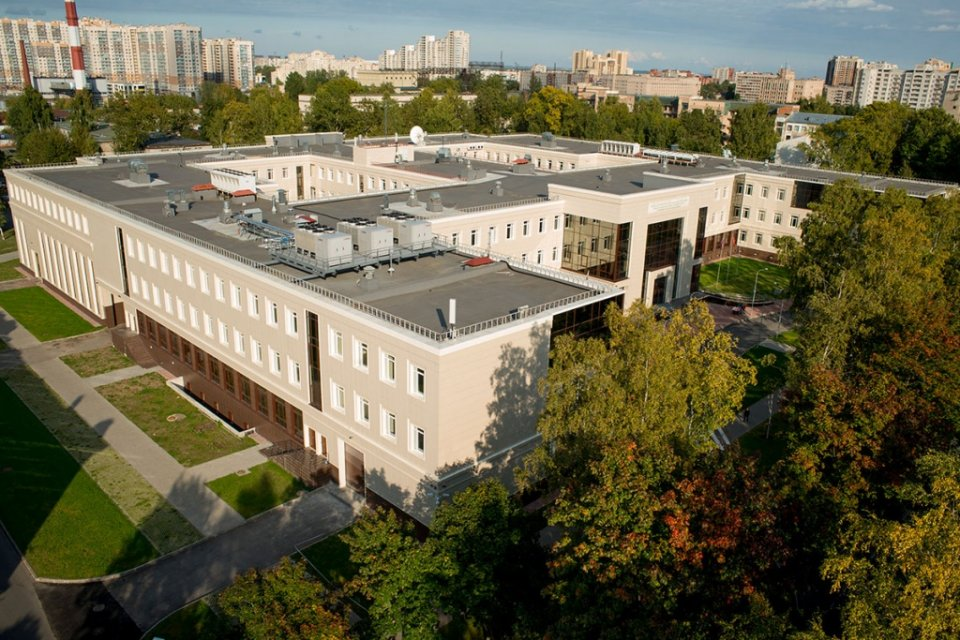
\includegraphics [scale=0.27] {my_folder/images/spbpu_new_bld_autumn}
	\caption{Новый научно-исследовательский корпус СПбПУ \cite{spbpu-gallery}} 
	\label{fig:spbpu-new-bld-autumn}  
	\end{figure}
	


		Пример представления данных в табличном виде приведён в таблице \ref{tab:ToyCompare-Peskov}.
	
	\begin{table} [htbp]% Пример записи таблицы с номером, но без отображаемого наименования
		\centering
		\caption{Пример задания данных в табличном виде из \cite{Peskov2004}}%
		\label{tab:ToyCompare-Peskov}		\begin{SingleSpace}
			%		\resizebox{1\linewidth}{!}{
			\begin{tabular}{|l|l|l|l|l|l|}
				\hline
				$G$&$m_1$&$m_2$&$m_3$&$m_4$&$K$\\
				\hline
				$g_1$&0&1&1&0&1\\
				$g_2$&1&2&0&1&1\\
				$g_3$&0&1&0&1&1\\
				$g_4$&1&2&1&0&2\\
				$g_5$&1&1&0&1&2\\
				$g_6$&1&1&1&2&2\\
				\hline		
			\end{tabular}	
			%		}
		\end{SingleSpace}
	\end{table}
		 % таблица с примером из \cite{Peskov2004}	

	
	\section{Название подраздела} \label{ch-11:sec-abbr} %название по-русски
	\addtocru{section}{Название подраздела} %повторите название по-русски
	\addtocen{section}{Section title} % title in english 
	
	
Название подраздела оформляется с помощью команды \verb|\section{...}|. В терминологии ГОСТов название главы является разделом (в \LaTeX{} команда \verb|\chapter{...}|). Для переноса названий структурных элементов глав (статей) в русское и английское содержание необходимо использовать команды \verb|\addtocru{element}{Название_на_русском}| и \verb|\addtocen{element}{Title_in_english}| соответственно, где под \verb|element| имеется в виду название структурного элемента издания, например, \verb|chapter|, \verb|section|.
	

	

	\subsection{Название параграфа} \label{ch-11:subsec-title-abbr} %название по-русски
	\addtocru{subsection}{Название параграфа} %повторите название по-русски
	\addtocen{subsection}{Paragraph title} % title in english 
	
	
Название параграфа оформляется с помощью команды  \texttt{\textbackslash{}subsection\{...\}}.
	
			
	\subsubsection{Название подпараграфа} \label{ch-11:subsubsec-title-abbr} %название по-русски
	\addtocru{subsubsection}{Название подпараграфа} %повторите название по-русски
	\addtocen{subsubsection}{Subparagraph title} % title in english 
	
	
Название подпараграфа оформляется с помощью команды  \texttt{\textbackslash{}subsubsecti\-on\{...\}}.



Перечисления могут использоваться с иерархией (как правило, {\itshape после параграфа или подпараграфа}) и без иерархии (в остальных случаях). Нумерационная часть при этом формируется следующим способом:

\begin{enumerate}[1.]
	\item В перечислениях {\itshape без иерархии} оформляется арабскими цифрами с точкой (или длинным тире).
	\item В перечислениях {\itshape с иерархией} --- в последовательности сначала прописных латинских букв с точкой, затем арабских цифр с точкой и далее --- строчных латинских букв со скобкой. 
\end{enumerate}


%% Если в дальнейшем нужно сделать сслыку на один из элементов нумеруемого перечисления, то нужно использовать конктрукцию типа:

%\begin{enumerate}[label=\arabic{enumi}.,ref=\arabic{enumi}]
%	\item text 1 \label{item:text1}
%	\item text 2
%\end{enumerate}
%\ref{item:text1}.


Далее приведён пример перечислений с иерархией.


\begin{enumerate}
	\item Первый пункт.
	\item Второй пункт.
	\item Третий пункт.
	\item По ГОСТ 2.105 первый уровень нумерации идёт буквами русского или латинского алфавитов ({\itshape для определенности выбираем английский алфавит}),
	а второй "--- цифрами. 
	\begin{enumerate}
		\item В данном пункте лежит следующий нумерованный список: 
		\begin{enumerate}
			\item первый пункт;
			\item третий уровень нумерации не нормирован ГОСТ 2.105 ({\itshape для определенности выбираем английский алфавит});
			\item обращаем внимание на строчность букв в этом нумерованном и следующем маркированном списке:
			\begin{itemize}
				\item первый пункт маркированного списка.
			\end{itemize}    
		\end{enumerate}
	\end{enumerate}
	\item Пятый пункт верхнего уровня перечисления.
\end{enumerate}

Маркированный список используется, если нет необходимости ссылки на определенное положение в списке:
\begin{itemize}
	\item первый пункт c {\itshape маленькой буквы} по правилам русского языка;
	\item второй пункт c {\itshape маленькой буквы} по правилам русского языка.
\end{itemize} % правила использования перечислений	

	
Оформление псевдокода необходимо осуществлять с помощью пакета \verb|algorithm2e| в окружении \verb|algorithm|. Данное окружение интерпретируется в шаблоне как рисунок. Пример оформления псевдокода алгоритма приведён на рисунке \ref{alg:AlgoFDSCALING}. 
	
	
	\begin{algorithm} %[h]
		\SetKwFunction{algoDTestsFDSCALING}{} 
		\SetKwProg{myalg}{Algorithm}{}{} %write in 2nd agrument <<Algorithm>>, <<Procedure>> etc
		\nonl\myalg{\algoDTestsFDSCALING}{
			\KwInput{the many-valued context $\cont[M]\eqdef(G,M,W,J)$, the class membership $\epsilon: G\to K$} 
			\KwOutput{positive and negative binary contexts $\overbar{\cont[K]_+}\eqdef(\overbar{G_+},M,I_+)$, $\overbar{\cont[K]_-}\eqdef(\overbar{G_-},M,I_-)$ such that i-tests found in $\overbar{\cont[K]_+}$ are diagnostic tests in $\cont[M]$, and objects from $\overbar{\cont[K]_-}$ are counter-examples} %последние строки формируют начальное множество диагностических тестов
			\For {$\forall g_i,$ $g_j \in G$\label{step:FD-scaling-first-step}}{
				%(\tcp*[f]{possible inlined comment})
				\If{$i < j$ }{
					$\overbar{G} \leftarrow (g_i,g_j)$\;
				}
			}
			%		$M\leftarrow M\setminus k$\;
			\For {$\forall (g_i,g_j)\in \overbar{G}$}{
				%(\tcp*[f]{possible inlined comment})
				\If{$m(g_i) = m(g_j)$ }{ %на самом деле здесь цикл по всем компонентам вектора-строки
					$(g_i,g_j) I m$\; % or setI() function
				}
				\uIf{$\epsilon(g_i) = \epsilon(g_j)$ }{
					$\overbar{G_+} \leftarrow (g_i,g_j)$\;
				}
				\lElse{$\overbar{G_-} \leftarrow (g_i,g_j)$\label{FD-scaling-step-last}}	
			}		
			$I_+= I\cap (\overbar{G_+}\times M)$, $I_-= I\cap (\overbar{G_-}\times M)$\label{FD-scaling-step-newK}\; 
			\For {$\forall \overbar{g_+}\in \overbar{G_+}$, $\forall \overbar{g_-}\in \overbar{G_-}$ }{
				\If{$\overbar{g_+}\uA \subseteq \overbar{g_-}\uA$ }{
					$\overbar{G_+} \leftarrow \overbar{G_+} \setminus \overbar{g_+}$\;
				}
			}
			%		\Return \;
		}
		\caption{Псевдокод алгоритма \texttt{DiagnosticTestsScalingAndInferring} \cite{Naidenova2017}}\label{alg:AlgoFDSCALING}
		% example of adding an item to Index
		% \index for accepted papers only
		\index[ru]{алгоритм!\texttt{название\_алгоритма}} 
		% key words <<алгоритм>> и <<algorithm>> keep unmodified
		\index[en]{algorithm!\texttt{algorighm\_title}}
		% authors can used the key word <<процедура>> (procedure) и т.п.
		%
		%
	    % another example:
		\index[ru]{алгоритм!\texttt{DiagnosticTestsScaling\-AndInferring}} %нужен ручной перенос \- из-за ошибки в MakeIndex для команды \texttt
		%ключевые слова <<алгоритм>> и <<algorithm>> не менять
		\index[en]{algorithm!\texttt{DiagnosticTestsScaling\-AndInferring}} %нужен ручной перенос \- из-за ошибки в MakeIndex для команды \texttt
	\end{algorithm} 
	
	% another example of adding an arbitrary keyword to Index
	% some useful keywords: theorem, proposition, lemma, equation etc
	% please, use short keywords (2-3 max)
	\index[ru]{длинное-название-возможное-например-на-немецком} % длинные названия первого уровня как правило запрещены
	\index[en]{long-title-possible-for-example-in-German} 
	
Обратим внимание, что можно сослаться на строчку \ref{step:FD-scaling-first-step} псевдокода из рисунка \ref{alg:AlgoFDSCALING}.  % пример оформления псевдокода алгоритма 	

	
	\section{Название подраздела} \label{ch-11:sec-very-short-title} %название по-русски
	\addtocru{section}{Название подраздела} %повторите название по-русски
	\addtocen{section}{Section title} % title in english  


	
Одиночные формулы также, как и отдельные формулы в составе группы, могут быть размещены в несколько строк. Чтобы выставить номер формулы напротив средней строки, используйте окружение \verb|multlined| из пакета \verb|mathtools| (вместо \verb|multline|) следующим образом \cite{Ganter1999}:

\begin{equation} % \tag{S} % tag - вписывает свой текст 
\label{eq:fConcept-order-G}
\begin{multlined}
(A_1,B_1)\leq (A_2,B_2)\; \Leftrightarrow \\  \Leftrightarrow\; A_1\subseteq A_2\; \Leftrightarrow \\ \Leftrightarrow\; B_2\subseteq B_1. 
\end{multlined}
\end{equation}

	
Используя команду \verb|\labelcref{...}| из пакета \verb|cleveref|, допустимо оформить ссылку на несколько формул, например, (\labelcref{eq:UpArrow-G,eq:DownArrow-G,eq:fConcept-order-G}). % пример оформления одиночной формулы в несколько строк

Пример оформления четырёх иллюстраций в одном текстово-графическом объекте приведён на рисунке \ref{fig:spbpu_sc-four-photos}. Это возможно благодаря использованию пакета \verb|subcaption|.

\begin{figure}[ht]
	\adjustbox{minipage=1.3em,valign=t}{\subcaption{}\label{fig:spbpu_sc-a}}%
	\begin{subfigure}[t]{\dimexpr.5\linewidth-1.3em\relax}
		\centering
		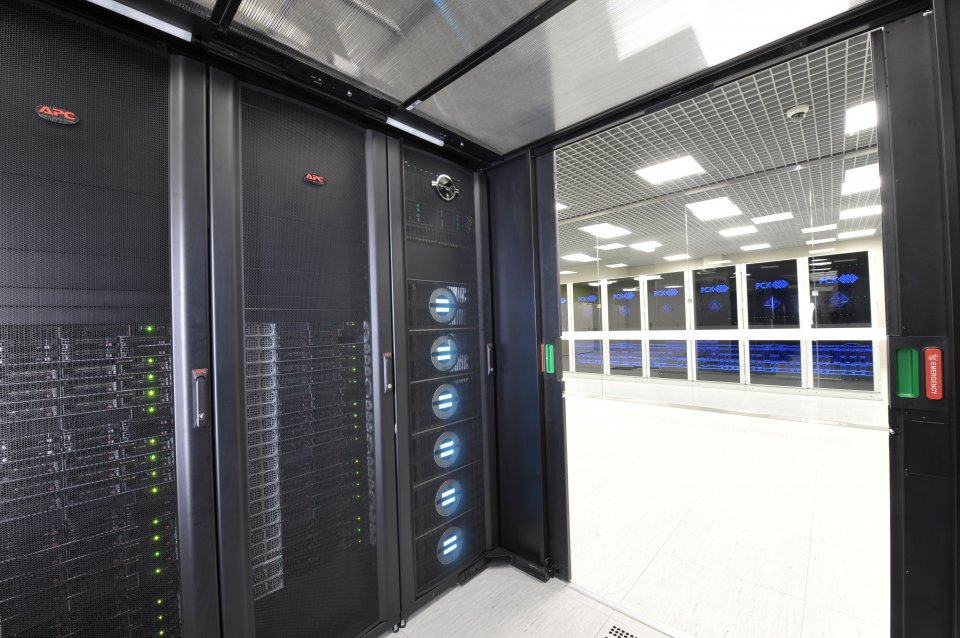
\includegraphics[width=.95\linewidth,valign=t]{my_folder/images/spbpu_sc_system}
	\end{subfigure}
\hfill %выровнять по ширине
	\adjustbox{minipage=1.3em,valign=t}{\subcaption{}\label{fig:spbpu_sc-b}}%
	\begin{subfigure}[t]{\dimexpr.5\linewidth-1.3em\relax}
		\centering
		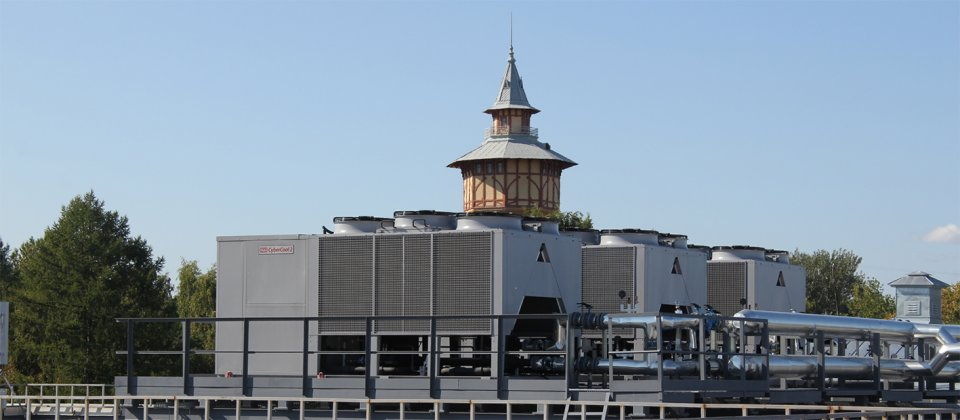
\includegraphics[width=.95\linewidth,valign=t]{my_folder/images/spbpu_sc_refr}
	\end{subfigure}
\\[20pt]
	\adjustbox{minipage=1.3em,valign=t}{\subcaption{}\label{fig:spbpu_sc-c}}%
\begin{subfigure}[t]{\dimexpr.5\linewidth-1.3em\relax}
	\centering
	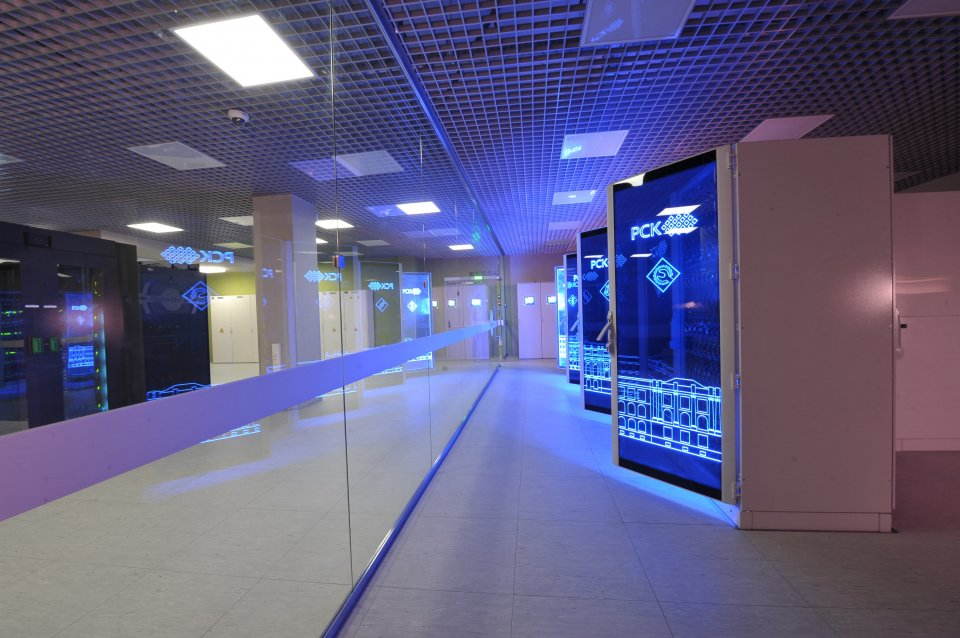
\includegraphics[width=.95\linewidth,valign=t]{my_folder/images/spbpu_sc_hall}
\end{subfigure}%
\hfill %выровнять по ширине
\adjustbox{minipage=1.3em,valign=t}{\subcaption{}\label{fig:spbpu_sc-d}}%
\begin{subfigure}[t]{\dimexpr.5\linewidth-1.3em\relax}
	\centering
	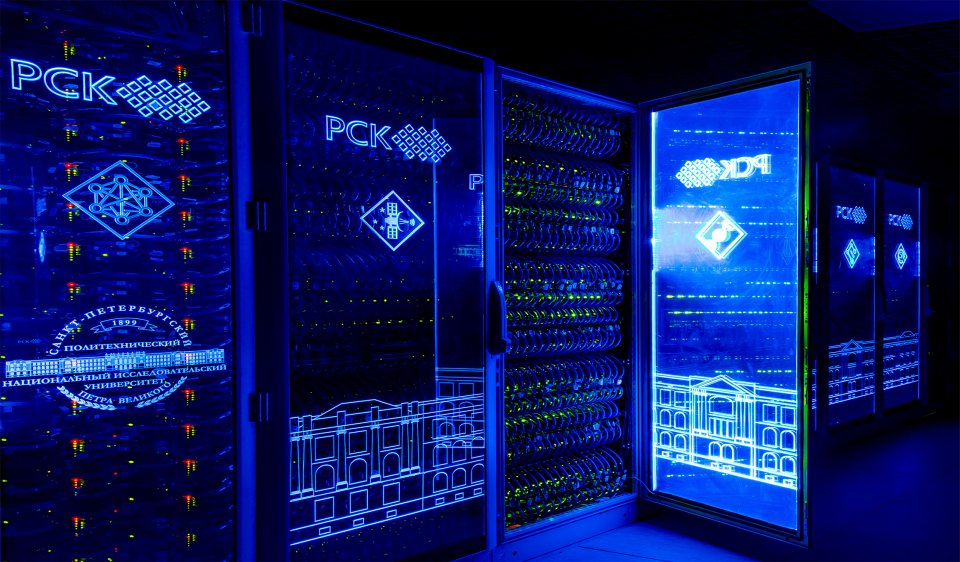
\includegraphics[width=.95\linewidth,valign=t]{my_folder/images/spbpu_sc_box}
\end{subfigure}
\captionsetup{justification=centering} %центрировать
\caption{Фотографии суперкомпьютерного центра СПбПУ \cite{spbpu-gallery}: {\itshape a} --- система хранения данных и узлы NUMA-вычислителя; {\itshape b} --- холодильные машины на крыше научно-исследовательского корпуса; {\itshape c} --- машинный зал; {\itshape d} --- элементы вычислительных устройств} 
\label{fig:spbpu_sc-four-photos}
\end{figure}

Далее можно ссылаться на рисунок \ref{fig:spbpu_sc-a}, \ref{fig:spbpu_sc-b}, \ref{fig:spbpu_sc-c}, \ref{fig:spbpu_sc-d} или на три из четырёх изображений одновременно: рисунки \labelcref{fig:spbpu_sc-a,fig:spbpu_sc-b,fig:spbpu_sc-c}. % пример подключения 4х иллюстраций в одном рисунке

%На рисунке \ref{fig:spbpu_whitehall-three-photos} приведены три картинки под~общим номером и~названием, но с раздельной нумерацией подрисунков посредством пакета \verb|subcaption|.

\begin{figure}[!htbp]
	\adjustbox{minipage=1.3em,valign=t}{\subcaption{}\label{fig:spbpu_whitehall-a}}%
	\begin{subfigure}[t]{\dimexpr.3\linewidth-1.3em\relax}
		\centering
		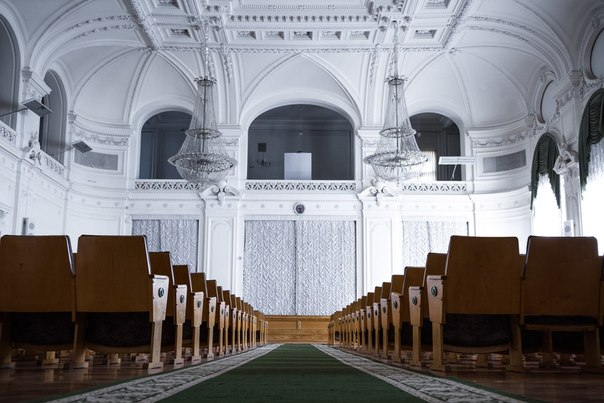
\includegraphics[width=.95\linewidth,valign=t]{my_folder/images//spbpu_whitehall}
	\end{subfigure}
	\hfill %выровнять
	\adjustbox{minipage=1.3em,valign=t}{\subcaption{}\label{fig:spbpu_whitehall-b}}%
	\begin{subfigure}[t]{\dimexpr.3\linewidth-1.3em\relax}
		\centering
		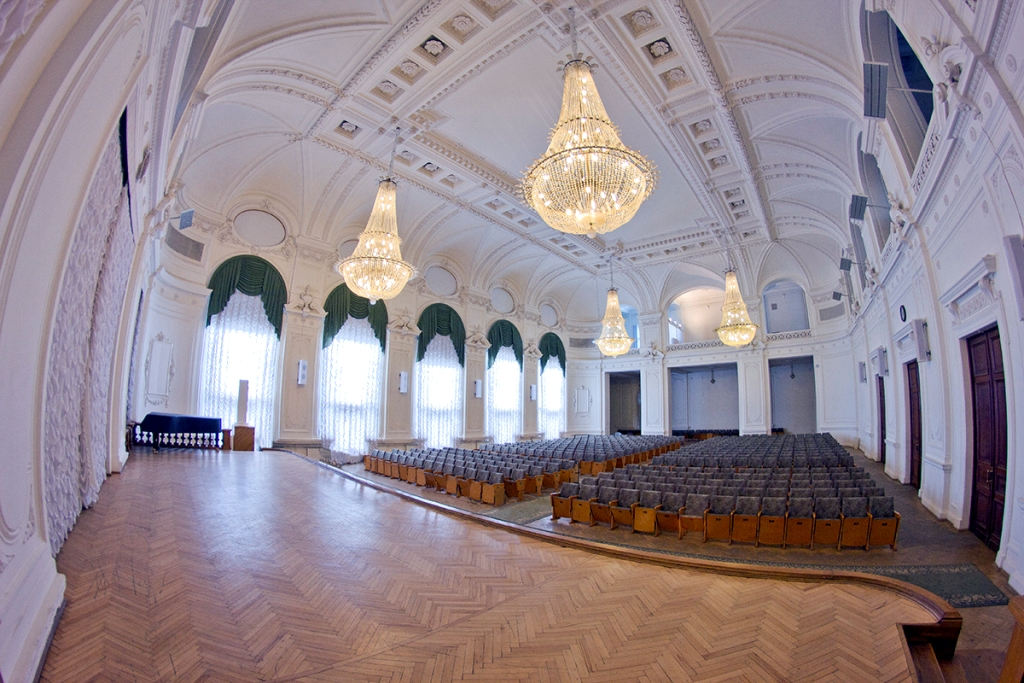
\includegraphics[width=.95\linewidth,valign=t]{my_folder/images//spbpu_whitehall_ligh}
	\end{subfigure}
	\hfill %выровнять
		\adjustbox{minipage=1.3em,valign=t}{\subcaption{}\label{fig:spbpu_whitehall-c}}%
	\begin{subfigure}[t]{\dimexpr.3\linewidth-1.3em\relax}
		\centering
		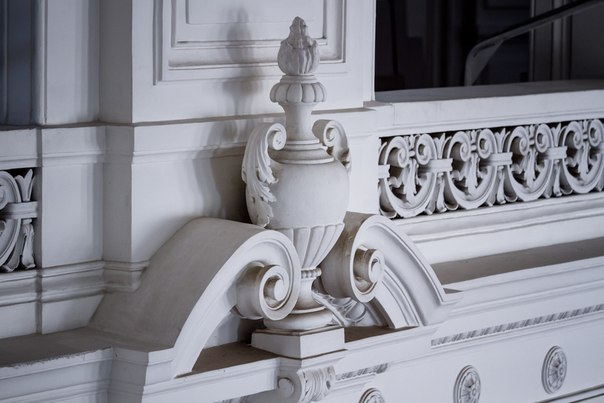
\includegraphics[width=.95\linewidth,valign=t]{my_folder/images//spbpu_whitehall_sculpture}
	\end{subfigure}%
\captionsetup{justification=centering} %центрировать
	\caption{Фотографии Белого зала СПбПУ \cite{spbpu-gallery}, в том числе: {\itshape a} --- со стороны зрителей; {\itshape b} --- со стороны сцены; {\itshape c} --- барельеф}\label{fig:spbpu_whitehall-three-photos}  
\end{figure}

Далее можно ссылаться на три отдельных рисунка \ref{fig:spbpu_whitehall-a}, \ref{fig:spbpu_whitehall-b} и \ref{fig:spbpu_whitehall-c}. % пример подключения 3х иллюстрации в одном рисунке
%
%На рисунке \ref{fig:spbpu_main_bld-two-photos} приведены две картинки под~общим номером и~названием.


\begin{figure}[!htbp]
	\adjustbox{minipage=1.3em,valign=t}{\subcaption{}\label{fig:spbpu_main_bld_entrance_autumn}}%
	\begin{subfigure}[t]{\dimexpr.5\linewidth-1.3em\relax} %разрешили выделить 0,5 стр в ширину на рисунок
		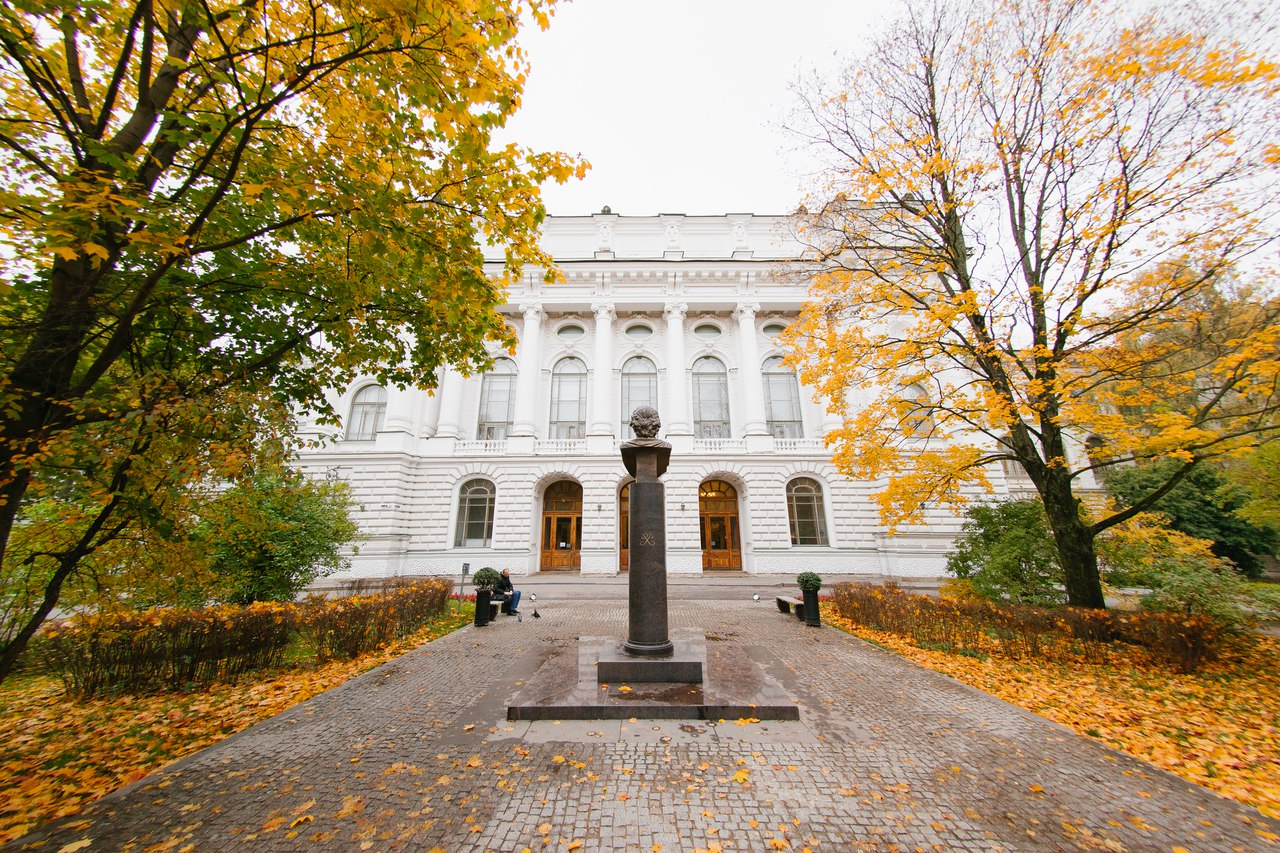
\includegraphics[height=0.20\textheight,valign=t]{my_folder/images//spbpu_main_bld_entrance_autumn} %высоту рисунка выставили как 0,3 от высоты наборного поля
	\end{subfigure}
%	\hfill %выровнять по ширине
	\adjustbox{minipage=1.3em,valign=t}{\subcaption{}\label{fig:spbpu_main_bld_whitehall}}%
	\begin{subfigure}[t]{\dimexpr.5\linewidth-1.3em\relax}%разрешили выделить 0,5 стр в ширину на рисунок
		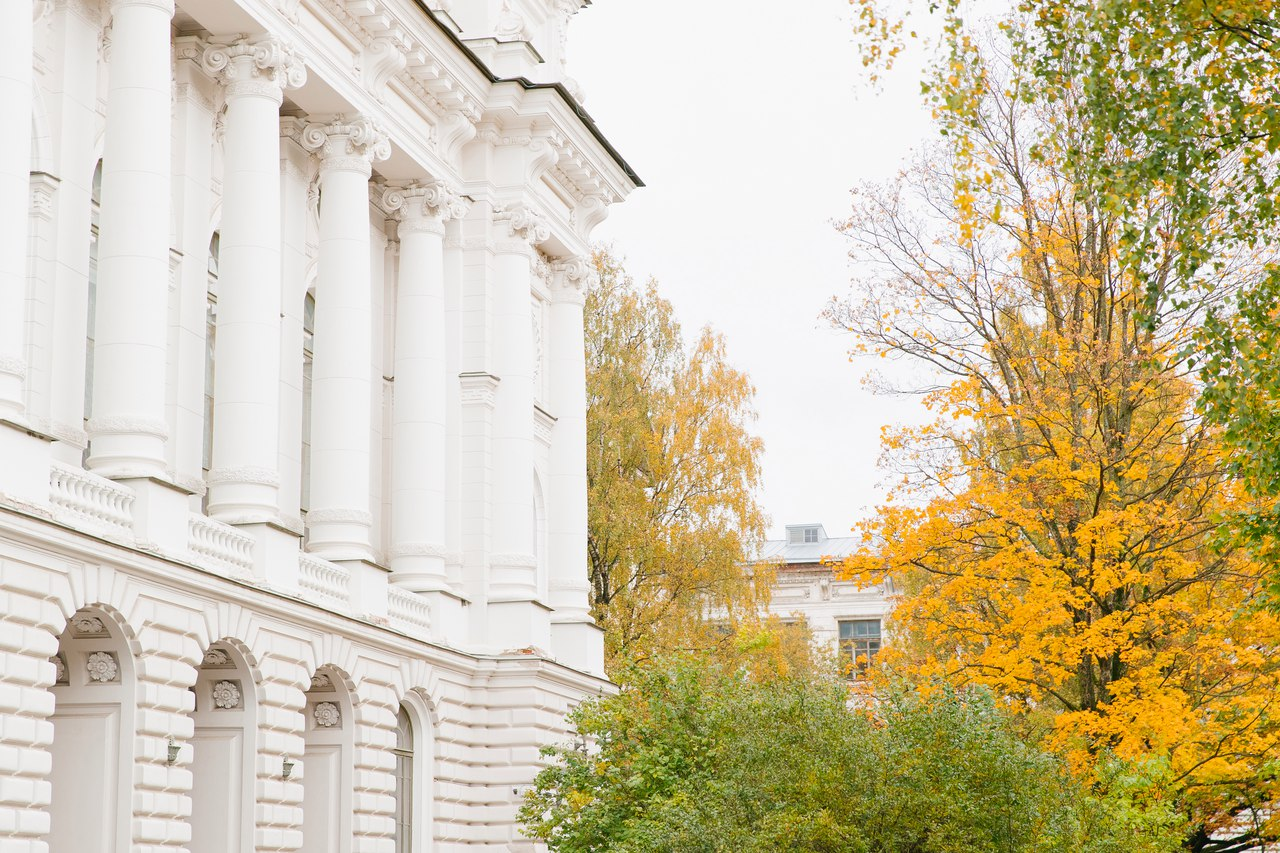
\includegraphics[height=0.20\textheight,valign=t]{my_folder/images//spbpu_main_bld_whitehall}%высоту рисунка выставили как 0,3 от высоты наборного поля
	\end{subfigure}
\captionsetup{justification=centering} %центрировать
	\caption{Вид на главное здание СПбПУ \cite{spbpu-gallery}, включая: {\itshape a} --- вход со стороны парка осенью; {\itshape b}~--- окна Белого зала}\label{fig:spbpu_main_bld-two-photos} 
\end{figure}

На рисунке \ref{fig:spbpu_main_bld_entrance_autumn} изображен вход со стороны парка СПбПУ осенью, а рисунке \ref{fig:spbpu_main_bld_whitehall}~--- окна Белого зала. % пример подключения 2х иллюстраций в одном рисунке

Приведём пример табличного представления данных с записью продолжения на следующей странице, см. таблицу \ref{tab:long}.

\begingroup
\centering
\smallA %выставляем шрифт в 13bp
\begin{longtable}[c]{|l|l|l|l|l|l|}
	\caption{Пример задания данных из \cite{Peskov2004} (с повтором для переноса таблицы на новую страницу)}%
	\label{tab:long}% label всегда желательно идти после caption
	\\
	\hline
	$G$&$m_1$&$m_2$&$m_3$&$m_4$&$K$\\ \hline
	\endfirsthead%
	\captionsetup{format=tablenocaption,labelformat=continued}% должен стоять до самого caption
	\caption[]{}\\
	\hline
	$G$&$m_1$&$m_2$&$m_3$&$m_4$&$K$\\ \hline
	\endhead
	\hline
	\endfoot
	\hline
	\endlastfoot
	$g_1$&0&1&1&0&1\\
	$g_2$&1&2&0&1&1\\
	$g_3$&0&1&0&1&1\\
	$g_4$&1&2&1&0&2\\
	$g_5$&1&1&0&1&2\\
	$g_6$&1&1&1&2&2\\
	\hline
	$g_1$&0&1&1&0&1\\
	$g_2$&1&2&0&1&1\\
	$g_3$&0&1&0&1&1\\
	$g_4$&1&2&1&0&2\\
	$g_5$&1&1&0&1&2\\
	$g_6$&1&1&1&2&2\\
	\hline
	$g_1$&0&1&1&0&1\\
	$g_2$&1&2&0&1&1\\
	$g_3$&0&1&0&1&1\\
	$g_4$&1&2&1&0&2\\
	$g_5$&1&1&0&1&2\\
	$g_6$&1&1&1&2&2\\
		\hline
	$g_1$&0&1&1&0&1\\
	$g_2$&1&2&0&1&1\\
	$g_3$&0&1&0&1&1\\
	$g_4$&1&2&1&0&2\\
	$g_5$&1&1&0&1&2\\
	$g_6$&1&1&1&2&2\\
	\hline
	$g_1$&0&1&1&0&1\\
	$g_2$&1&2&0&1&1\\
	$g_3$&0&1&0&1&1\\
	$g_4$&1&2&1&0&2\\
	$g_5$&1&1&0&1&2\\
	$g_6$&1&1&1&2&2\\
\end{longtable}
\normalsize% возвращаем шрифт к нормальному
\endgroup
\normalsize% возвращаем шрифт к нормальному % пример подключения таблицы на несколько страциц



%% please, before using, read the author guide carefully

%\noindent % for correct centering
\begin{minipage}{\textwidth}
	\vspace{\mfloatsep} % интервал 
	\centering
	\captionof{table}{Пример задания данных в табличном виде из \cite{Peskov2004} (с помощью окружения minipage)}%
	\label{tab:ToyCompare-Peskov-minipage}
\begin{SingleSpace}
\begin{tabular}{|l|l|l|l|l|l|}
	\hline
	$G$&$m_1$&$m_2$&$m_3$&$m_4$&$K$\\
	\hline
	$g_1$&0&1&1&0&1\\
	$g_2$&1&2&0&1&1\\
	$g_3$&0&1&0&1&1\\
	$g_4$&1&2&1&0&2\\
	$g_5$&1&1&0&1&2\\
	$g_6$&1&1&1&2&2\\
	\hline		
\end{tabular}
\end{SingleSpace}
\vspace{\mfloatsep} % интервал  	
\end{minipage} % пример подключения minipage

%\noindent % for correct centering
\begin{minipage}{\textwidth}
	\centering
	\vspace{\mfloatsep} % интервал  	
	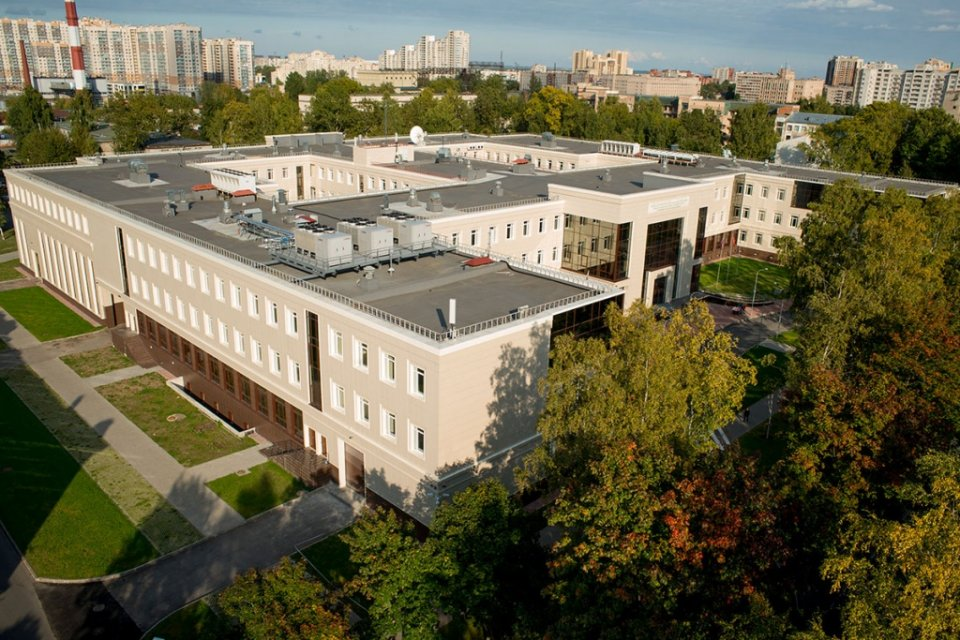
\includegraphics[keepaspectratio=true,scale=0.27] {my_folder/images/spbpu_new_bld_autumn}
	\captionof{figure}{Новый научно-исследовательский корпус СПбПУ \cite{spbpu-gallery} (с помощью окружения minipage)}\label{fig:spbpu-new-bld-autumn-minipage}  
	\vspace{\mfloatsep} % интервал  	
\end{minipage} % пример подключения minipage




Вопросы форматирования текстово-графических объектов (окружений) не регламентированы в известных нам ГОСТах, поэтому предлагаем придерживаться следующих правил:

\begin{itemize}
	\item \textbf{полужирный текст} рекомендуем использовать только для названий стандартных окружений с нумерационной частью, например, \textbf{определение 1.1}, \textbf{теорема 2.2}, \textbf{пример 2.3}, \textbf{лемма 4.5};
	
	\item \textit{курсив} рекомендуем использовать только для выделения переменных в формулах, служебной информации об авторах главы (статьи), важных терминов, представляемых по тексту, а также для всего тела окружений, связанных с получением \textit{новых существенных результатов и их доказательством}: теорема, лемма, следствие, утверждение и другие.
\end{itemize}

 

По аналогии с нумерацией формул, рисунков и таблиц нумеруются и иные текстово-графические объекты, то есть включаем в нумерацию номер главы, например: теорема 3.1. для первой теоремы третьей главы монографии. Команды \LaTeX{} выставляют нумерацию и форматирование автоматически. Полный перечень команд для подготовки текстово-графических и иных объектов находится в подробных методических рекомендациях \cite{spbpu-bci-template-author-guide}. 


%Для удобства авторов некоторые названия стандартных окружений приведены в таблице \ref{tab:enum-std}. В таблице \ref{tab:enum-spbpu}  перечислены имена специально разработанных окружений для пакетов SPbPU.

% и примеры их оформления на псевдокоде (см. \cite{cite-spbpu-bci}).


%https://tex.stackexchange.com/questions/2651/should-i-use-center-or-centering-for-figures-and-tables


	\begin{table} [htbp]% Пример записи таблицы с номером, но без отображаемого наименования
	\centering
	\caption{Описание некоторых стандартных \LaTeX{} окружений, рекомендуемых к использования в шаблонах SPbPU}%
	\label{tab:enum-std}
		\begin{SingleSpace}
		%		\resizebox{1\linewidth| &!| &
		\begin{tabular}{|l|p{11cm}|} 
			\hline
			Название окружения&Назначение\\
			\hline
			\verb|center| & центрирование, аналог команды \verb|\centering|, но с добавлением нежелательного пробела, поэтому лучше избегать применения \verb|center|; \\
			\verb|itemize| &{перечисления, в которых нет необходимости нумеровать  пункты, см. подробнее подраздел \ref{sec:strct-and-enum};}\\
			\verb|enumerate| & перечисления с нумерацией, см. подробнее подраздел \ref{sec:strct-and-enum}; \\
			\verb|refsection| & создание отдельных библиографических списков для глав; \\
			\verb|tabular| & оформление таблиц; \\
			\verb|table|   &{автоматическое перемещение по тексту таблиц, оформленных, например, с помощью \verb|tabular|, для минимизации пустых пространств;} \\
			\verb|longtable| & оформление многостраничных таблиц; \\
			\verb|tikzpicture| & создание иллюстраций с помощью пакета \verb|tikz| \cite{ctan-tikz}; \\
			\verb|figure| &{автоматическое перемещение по тексту рисунков, оформленных например, с помощью \verb|tikz| или подключенных с помощью команды \verb|\includegraphics|, для минимизации пустых пространств;}\\
			\verb|subfigure| & оформление вложенных рисунков в составе \verb|figure|; \\
			\verb|algorithm| &{оформление псевдокода на основе пакета \verb|algorithm2e| \cite{ctan-algorithm2e};} \\
			\verb|minipage| & {оформление рисунков и таблиц без функций автоматического перемещения по тексту для  минимизации пустых пространств;} \\
			\verb|equation| & {оформление выключенных (не встроенных в текст с помощью \verb|$...$|) одиночных формул на одной строке;} \\
			\verb|multilined| &{оформление выключенных (не встроенных в текст с помощью \verb|$...$|) одиночных формул в несколько строк;} \\ 
			\verb|aligned| &{оформление нескольких формул с выравниванием по символу \verb|&|.} \\
			\hline		
		\end{tabular}	
		%		}
	\end{SingleSpace}
	\end{table}

На базе пакета \verb|tikz| разработано большое количество расширений \cite{ctan-tikz}, например, \verb|tikzcd|, которые мы рекомендуем использовать для оформления иллюстраций.

	\begin{table} [htbp]% Пример записи таблицы с номером, но без отображаемого наименования
	\centering
	\caption{Описание специально разработанных \LaTeX{} окружений, рекомендуемых к использования в шаблонах SPbPU}%
	\label{tab:enum-spbpu}
	\begin{SingleSpace}
		%		\resizebox{1\linewidth| &!| &
		\begin{tabular}{|l|l|}
			\hline
			Название окружения & Текстово-графический объект\\
			\hline
			\verb|abstr|	 & реферат (abstract); \\
			\verb|m-theorem| & теорема; \\ 
			\verb|m-corollary| & следствие; \\
			\verb|m-proposition| & утверждение; \\
			\verb|m-lemma|   & лемма; \\
			\verb|m-axiom| & аксиома; \\
			\verb|m-example| & пример; \\
			\verb|m-definition| &  определение; \\
			\verb|m-condition| & условие;\\
			\verb|m-problem| & проблема; \\
			\verb|m-exercise| & упраженение;\\
			\verb|m-question| & вопрос;\\
			\verb|m-hypothesis| & гипотеза;\\
			\verb|m-task| & задание. \\
			\hline		
		\end{tabular}	
		%		}
	\end{SingleSpace}
\end{table}

В случае, если авторам потребовалось новое окружение, то создать его можно в файле в файле \texttt{my\_fol\-der/{}my\_set\-tings.tex} согласно правилам, приведённым ниже.

\begin{enumerate}[1.]
	\item Для перехода в режим создания окружений следует указать:
	\begin{itemize}
		\item \verb|\theoremstyle{myplain}| --- окружения с доказательствами или аксиомами;
		\item \verb|\theoremstyle{mydefinition}| --- окружения, не связанные с доказательствами или аксиомами.
	\end{itemize}
	\item В команде создания окружения следует ввести краткий псевдоним (\verb|m-new-env|) и отображаемое в pdf имя окружения (\verb|Название_окружения|):
	\begin{itemize}
		\item \texttt{\textbackslash{}newtheorem\{m-new-env-second\}\{Название\_окруже\-ния\}\-[chap\-ter]}.
	\end{itemize}
\end{enumerate}


%\begin{m-new-env-first}
%	Тест первого пользовательского окружения
%\end{m-new-env-first}
%
%\begin{m-new-env-second}
%	Тест второго пользовательского окружения
%\end{m-new-env-second} % список некоторых окружений


\begin{m-theorem}[о неполноте] %при необходимости в [] можно записать название теоремы или убрать его
	\label{th:ex} 
	% \index только для принятых работ
	% шаблон записи теоремы в Предметный указатель
	\index[ru]{теорема!название\_теоремы или о чём} %ключевое слово <<теорема>> не менять
	\index[en]{theorem!1-3 words for detail or description}
	% пример записи алгоритма в Предметный указатель
	\index[ru]{теорема!о неполноте}
	\index[en]{theorem!about incompleteness}
	% пример записи алгоритма в Предметный указатель
	\index[ru]{теорема!о жизни}
	\index[en]{theorem!about life}
	Текст теоремы полностью выделен курсивом. Допустимо математические символы не выделять курсивом, если это искажает их значения. Используется абзацный отсуп, так как ``Абзацы в тексте начинают отступом'' в соответствии с ГОСТ 2.105--95. Название теоремы допустимо убрать.
\end{m-theorem}
Доказательство теоремы \ref{th:ex}, леммы, утверждений, следствий и других завершаем символом белого квадрата (номер символа в Юникод 25A1) без выравнивания по правому краю. $\square$

Тело доказательства не выделяется курсивом.
Тело следующих окружений также не выделяется сплошным курсивом: определение, условие, проблема, пример, упражнение, вопрос, гипотеза и другие. %пример оформления теоремы


\begin{m-definition}[хороший и-тест] %при необходимости в [] можно записать название определения или убрать его
	\label{def:ex}
	% \index только для принятых работ
	% шаблон записи определения в Предметный указатель 
	\index[ru]{название\_определения!1-3 уточняющих слова или~ничего}
	\index[en]{definition\_title!1-3 words for detail or~without "!-part}
	% пример записи определения в Предметный указатель 
	\index[ru]{и-тест!хороший!наилучший}
	\index[en]{i-test!good!best}
	% пример записи определения в Предметный указатель 
	\index[ru]{и-тест!замкнутый}
	\index[en]{i-test!closed}
	В тексте определения только {\itshape важные термины} выделяются курсивом. Если определение носит лишь вспомогательный характер, то допустимо не использовать окружение \texttt{m-definition}, представляя текст определения в обычном абзаце. Ключевые термины при этом обязательно выделяются курсивом.
\end{m-definition} %пример оформления определения



% пример повторной ссылки на алгоритм для записи упоминанаия определения в Предметный указатель на другой странице 
\index[ru]{алгоритм!\texttt{DiagnosticTestsScaling\-AndInferring}} %нужен ручной перенос \- из-за ошибки в MakeIndex для команды \texttt
%ключевые слова <<алгоритм>> и <<algorithm>> не менять
\index[en]{algorithm!\texttt{DiagnosticTestsScaling\-AndInferring}} %нужен ручной перенос \- из-за ошибки в MakeIndex для команды \texttt


\section*{Выводы} \label{ch-11:conclusion}

Текст заключения ко второй главе. Пример ссылок \cite{Article,Book,Booklet,Conference,Inbook,Incollection,Manual,Mastersthesis,Misc,Phdthesis,Proceedings,Techreport,Unpublished,badiou:briefings}, а также ссылок с указанием страниц, на котором отображены те или иные текстово-графические объекты  \cite[с.~96]{Naidenova2017} или в виде мультицитаты на несколько источников \cites[с.~96]{Naidenova2017}[с.~46]{Ganter1999}. Часть библиографических записей носит иллюстративный характер и не имеет отношения к реальной литературе.


\section*{Библиографический список}
\FloatBarrier % make floats stop


	
\printbibliography
\end{refsection}  
\newpage % keep unmodified